\documentclass[]{beamer}
\usepackage[T1]{fontenc}
\usepackage[utf8]{inputenc}
\usepackage{lmodern}
\usepackage[italian]{babel}
\usepackage{mathrsfs}
\usepackage{cancel}



\title{Ripasso: la meccanica newtoniana}
\author{\texorpdfstring{Mattia Cozzi\newline\href{mailto:cozzimattia@gmail.com}{\texttt{cozzimattia@gmail.com}}}{Mattia Cozzi}}
\date{a.s.~2023/2024}

%\documentclass[handout]{beamer}     %usare questa classe per generare l'handout
%\usepackage{pgfpages}   %per mostrare più quadri nella stessa pagina
%\pgfpagesuselayout{4 on 1}[a4paper,border shrink=5mm,landscape]
\usetheme{Singapore}
%\useoutertheme[left]{sidebar} %elementi intorno alle diapositive
\setbeamercovered{dynamic} %modifica l'aspetto del testo grigetto delle diapositive future. Argomenti: invisible/transparent/dynamic
\usecolortheme{orchid}
%COLORE PRINCIPALE
% \definecolor{marroncino}{RGB}{156, 26, 0} % UBC Blue (primary)
% \setbeamercolor{structure}{fg=marroncino} % itemize, enumerate, etc

\theoremstyle{plain}
\newtheorem{teorema}{Teorema}

\usepackage{tikz}
\usepackage{circuitikz}

\usepackage{pgf,pgfplots,graphicx}
\usetikzlibrary{angles,quotes,arrows,shapes,decorations.markings}
\pgfplotsset{compat=1.15}
\usepgfplotslibrary{units,fillbetween} % to add units easily to axis

\newcommand{\fem}{f_{em}}

\def\angolo[#1](#2)(#3:#4:#5)% Syntax: [draw options] (center) (initial angle:final angle:radius)
    { \draw[#1] ($(#2)+({#5*cos(#3)},{#5*sin(#3)})$) arc (#3:#4:#5); }


\begin{document}

\begin{frame}
  \titlepage
\end{frame}





\begin{frame}
\frametitle{Contenuti}
\tableofcontents
\end{frame}






\section{Cinematica}

\begin{frame}
\frametitle{Sistema di riferimento e legge oraria}
Per descrivere un moto, avremo \alert<1>{sempre} bisogno di esplicitare un sistema di riferimento, ovvero:\pause
\begin{itemize}
  \item stabilire un certo punto come \alert<2>{origine del sistema di riferimento} (valore zero dello spazio);\pause
  \item stabilire il \alert<3>{verso degli assi}, così da poter determinare il segno delle quantità coinvolte.
\end{itemize}\pause

~

\begin{block}{Legge oraria di un moto}
La legge oraria di un moto è una funzione $ s(t) $ che ad ogni istante di tempo associa una posizione del corpo nel sistema di riferimento.
\end{block}
\end{frame}


\begin{frame}
\frametitle{Velocità}
Se un corpo si muove lungo una retta e percorre uno spazio $ \Delta s $ in un tempo $ \Delta t $, definiamo la sua \alert{velocità media} come:
\begin{center}
\colorbox{blue!30}{$ \overline{v} = \dfrac{\Delta s}{\Delta t} = \dfrac{s_{2} - s_1}{\Delta t} $}~~~~~~~$ \left[ \dfrac{m}{s} \right] $
\end{center}
\end{frame}





\begin{frame}
  \frametitle{Moto rettilineo uniforme}
  \visible<1->{È il moto che si ottiene quando la somma delle forze agenti su un corpo è nulla.}\visible<2->{ Avviene a \alert{velocità costante} e lungo una \alert{linea retta}.}\\~
  \begin{columns}
\begin{column}{0.6\textwidth}
\visible<3->{Indichiamo con:
\begin{itemize}
  \item $ t $ = l'istante di tempo;}
  \visible<4->{\item $ v $ = la velocità del moto;}
  \visible<5->{\item $ s_0 $ = la posizione iniziale del corpo nel SDR;}
  \visible<6->{\item $ s(t) $ = la posizione del corpo all'istante $ t $.}
\end{itemize}
\end{column}
\begin{column}{0.3\textwidth}
\visible<7->{
\begin{center}
Legge oraria\\~\\
\colorbox{blue!30}{$ s(t) = vt + s_0  $}
\end{center}}
\end{column}
\end{columns}
\end{frame}


\begin{frame}
\frametitle{MRU sul piano spazio/tempo (1)}
\begin{center}
Confronta \colorbox{blue!30}{$ s(t) = vt + s_0 $} con \colorbox{blue!30}{$ y=mx + q $}.
\end{center}

\begin{columns}
\begin{column}{0.3\textwidth}
\begin{figure}\centering
\begin{tikzpicture}[scale=0.3]
\draw [->] (-1,0) -- (7,0);
\draw [->] (0,-1) -- (0,7);
\node [below] at (7,0) {$ t $};
\node [left] at (0,7) {$ s  $};
\draw [thick,red] (0,2) -- (7,5);
\end{tikzpicture}
\end{figure}
\begin{center}
$ v>0 $, $ s_0 \neq 0 $
\end{center}
\end{column}
\begin{column}{0.3\textwidth}
\begin{figure}\centering
\begin{tikzpicture}[scale=0.3]
\draw [->] (-1,0) -- (7,0);
\draw [->] (0,-1) -- (0,7);
\node [below] at (7,0) {$ t $};
\node [left] at (0,7) {$ s $};
\draw [thick,blue] (0,5) -- (7,2);
\end{tikzpicture}
\end{figure}
\begin{center}
$ v<0 $, $ s_0 \neq 0 $
\end{center}
\end{column}
\begin{column}{0.3\textwidth}
\begin{figure}\centering
\begin{tikzpicture}[scale=0.3]
\draw [->] (-1,0) -- (7,0);
\draw [->] (0,-1) -- (0,7);
\node [below] at (7,0) {$ t $};
\node [left] at (0,7) {$ s $};
\draw [thick,green] (0,0) -- (7,4);
\end{tikzpicture}
\end{figure}
\begin{center}
$ v>0 $, $ s_0 = 0 $
\end{center}
\end{column}
\end{columns}

~

~

Attenzione! Il grafico spazio/tempo non indica una \emph{traiettoria}!
\end{frame}


\begin{frame}
\frametitle{Esercizio}
\begin{exampleblock}{Posizione e istante di tempo}
  \small{Un gatto si muove con velocità costante $ v = - 1,4 \, \frac{m}{s} $ lungo una linea orientata partendo dalla posizione $ s_0 = +3,5 \, m $. 

  Dove si trova dopo $ 4,0 \, s $? In quante istante passa dall'origine?}
\end{exampleblock}
\end{frame}



\begin{frame}
\frametitle{MRU sul piano spazio/tempo (2)}


\begin{columns}
\begin{column}{0.3\textwidth}
\begin{figure}\centering
\begin{tikzpicture}[scale=0.3]
\draw [->] (-1,0) -- (7,0);
\draw [->] (0,-1) -- (0,7);
\node [below] at (7,0) {$ t $};
\node [left] at (0,7) {$ s  $};
\draw [thick,red] (0,2) -- (7,5);
\draw [thick,blue] (0,2) -- (7,3);
\end{tikzpicture}
\end{figure}
{\small I due corpi hanno la stessa direzione e punto di partenza, ma velocità diverse.}
\end{column}
\begin{column}{0.3\textwidth}
\begin{figure}\centering
\begin{tikzpicture}[scale=0.3]
\draw [->] (-1,0) -- (7,0);
\draw [->] (0,-1) -- (0,7);
\node [below] at (7,0) {$ t $};
\node [left] at (0,7) {$ s  $};
\draw [thick,red] (0,2) -- (7,4);
\draw [thick,blue] (0,1) -- (7,5);
\end{tikzpicture}
\end{figure}
{\small I due corpi hanno la stessa direzione, ma diversi punti di partenza e velocità.}
\end{column}
\begin{column}{0.3\textwidth}
\begin{figure}\centering
\begin{tikzpicture}[scale=0.3]
\draw [->] (-1,0) -- (7,0);
\draw [->] (0,-1) -- (0,7);
\node [below] at (7,0) {$ t $};
\node [left] at (0,7) {$ s  $};
\draw [thick,red] (0,5) -- (7,2);
\draw [thick,blue] (0,0) -- (7,5);
\end{tikzpicture}
\end{figure}
{\small I due corpi hanno punti di partenza diversi e velocità opposte.}
\end{column}\end{columns}
\end{frame}


\begin{frame}
\frametitle{MRU sul piano velocità/tempo}
\begin{center}
\colorbox{blue!30}{$ v(t) = v  $}
\end{center}
\begin{columns}
\begin{column}{0.3\textwidth}
\begin{figure}\centering
\begin{tikzpicture}[scale=0.3]
\draw [->] (-1,0) -- (7,0);
\draw [->] (0,-2) -- (0,7);
\node [below] at (7,0) {$ t $};
\node [left] at (0,7) {$ v $};
\draw [thick,red] (0,2) -- (6,2);
\end{tikzpicture}
\end{figure}
\begin{center}
$ v>0 $
\end{center}
\end{column}
\begin{column}{0.3\textwidth}
\begin{figure}\centering
\begin{tikzpicture}[scale=0.3]
\draw [->] (-1,0) -- (7,0);
\draw [->] (0,-2) -- (0,7);
\node [below] at (7,0) {$ t $};
\node [left] at (0,7) {$ v $};
\draw [thick,orange] (0,0) -- (6,0);
\end{tikzpicture}
\end{figure}
\begin{center}
$ v=0 $
\end{center}
\end{column}
\begin{column}{0.3\textwidth}
\begin{figure}\centering
\begin{tikzpicture}[scale=0.3]
\draw [->] (-1,0) -- (7,0);
\draw [->] (0,-2) -- (0,7);
\node [below] at (7,0) {$ t $};
\node [left] at (0,7) {$ v $};
\draw [thick,green] (0,-1) -- (6,-1);
\end{tikzpicture}
\end{figure}
\begin{center}
$ v<0 $
\end{center}
\end{column}
\end{columns}
\end{frame}


\begin{frame}
\frametitle{Esercizio}
\begin{exampleblock}{Incontro}
  \small{Marco e Anna abitano a $ 180 \, m $ di distanza. Partono dalle loro case contemporaneamente camminando in linea retta l'uno verso l'altro. Marco ha una velocità costante di $ 2,00 \, \frac{m}{s} $ e Anna di $ 2,80 \, \frac{m}{s} $.

Rappresenta i loro moti sul piano spazio/tempo e su quello velocità/tempo.

Dopo quanto tempo si incontrano? A che distanza dalla casa di Anna si incontrano?}
\end{exampleblock}
\end{frame}


\begin{frame}
  \frametitle{Consigli (direttive) per gli esercizi}
  
  \begin{itemize}
    \item Stabilire sempre con chiarezza un \alert{sistema di riferimento}, indicandone l'origine e il verso degli assi;\pause
    \item ricordarsi che il verso degli assi stabilito determina il \alert{segno} delle quantità in gioco;\pause
    \item esprimere ciò che si vuole imporre al sistema fisico mediante equazioni, sistemi di equazioni e assegnazione di valori alle quantità coinvolte;\pause
    \item svolgere \alert{prima} la parte algebrica dell'esercizio (facendo i calcoli con le lettere), e solo quando si è ottenuta la formula che fornisce la soluzione sostituire le lettere con il loro valore;\pause
    \item effettuare sempre i calcoli con le \alert{unità di misura} e con la \alert{notazione scientifica}.
  \end{itemize}
\end{frame}



\begin{frame}
\frametitle{Accelerazione}
Se un corpo si muove lungo una retta e la sua velocità varia da $ v_1 $ a $ v_2 $ un in un tempo $ \Delta t $, definiamo la sua \alert{accelerazione media} come:
\begin{center}
\colorbox{blue!30}{$ \overline{a} = \dfrac{\Delta v}{\Delta t} = \dfrac{v_2 -v_1}{\Delta t} $}~~~~~~~$ \left[ \dfrac{m}{s^2} \right] $
\end{center}
\end{frame}



\begin{frame}
\frametitle{Esercizio}
\begin{exampleblock}{Calcolo dell'accelerazione}
  \small{Una vettura di Formula 1 può passare da $ 328 \, \frac{km}{h} $ a $ 80 \, \frac{km}{h} $ in un tempo di $ 2,9 \, s $.
  
  Calcola il valore dell'accelerazione subita da un pilota. Esprimi successivamente tale accelerazione in funzione di $ g = 9,81 \, \frac{m}{s^2}$.}
\end{exampleblock}
\end{frame}




\begin{frame}
  \frametitle{Moto uniformemente accelerato}
  \visible<1->{È il moto che si ottiene quando la somma delle forze agenti su un corpo è diversa da zero.}\visible<2->{ Avviene ad \alert{accelerazione costante} e lungo una \alert{linea retta}.}\\~
  \begin{columns}
\begin{column}{0.6\textwidth}
\visible<3->{Indichiamo con:
\begin{itemize}
  \item $ a $ = l'accelerazione del corpo;}
  \visible<4->{\item $ v_0 $ = la velocità iniziale del corpo;}
  \visible<5->{\item $ s_0 $ = la posizione iniziale del corpo nel SDR;}
  \visible<6->{\item $ s(t) $ = la posizione del corpo all'istante $ t $.}
\end{itemize}
\end{column}
\begin{column}{0.3\textwidth}
\visible<7->{
\begin{center}
Legge oraria\\~\\
\colorbox{blue!30}{$ s(t) = \dfrac{1}{2} at^2 + v_0 t + s_0  $}
\end{center}}
\end{column}
\end{columns}
\end{frame}







\begin{frame}
  \frametitle{MUA sul piano spazio/tempo}
\begin{center}
Confronta \colorbox{blue!30}{$ s(t) = \frac{1}{2} at^2 + v_0 t + s_0 $} con \colorbox{blue!30}{$ y= ax^2 + bx + c $}.
\end{center}

\begin{columns}
\begin{column}{0.3\textwidth}
\begin{figure}\centering
\begin{tikzpicture}[scale=0.3]
\draw [->] (0,0) -- (7,0);
\draw [->] (0,0) -- (0,7);
\node [below] at (7,0) {$ t $};
\node [left] at (0,7) {$ s  $};
\draw [thick,red] (0,0) parabola (7,6);
\end{tikzpicture}
\end{figure}
\begin{center}
$ a >0 $\\$ v_0 = 0 $\\$ s_0 = 0 $
\end{center}
\end{column}
\begin{column}{0.3\textwidth}
\begin{figure}\centering
\begin{tikzpicture}[scale=0.3]
\draw [->] (0,0) -- (7,0);
\draw [->] (0,0) -- (0,7);
\node [below] at (7,0) {$ t $};
\node [left] at (0,7) {$ s  $};
\draw [thick,blue] (0,6) parabola (7,1);
\end{tikzpicture}
\end{figure}
\begin{center}
$ a <0 $\\$ v_0 = 0 $\\$ s_0 \neq 0 $
\end{center}
\end{column}
\begin{column}{0.3\textwidth}
\begin{figure}\centering
\begin{tikzpicture}[scale=0.3]
\draw [->] (0,0) -- (7,0);
\draw [->] (0,0) -- (0,7);
\node [below] at (7,0) {$ t $};
\node [left] at (0,7) {$ s $};
\draw [thick,green] (0,2) parabola bend (3,5) (7,0);
\end{tikzpicture}
\end{figure}
\begin{center}
$ a<0 $\\$ v_0 >0 $\\$ s_0 \neq 0 $
\end{center}
\end{column}
\end{columns}
\end{frame}


\begin{frame}
\frametitle{MUA sul piano velocità/tempo}
\begin{center}
\colorbox{blue!30}{$ v(t) = at + v_0  $}
\end{center}
\begin{columns}
\begin{column}{0.3\textwidth}
\begin{figure}\centering
\begin{tikzpicture}[scale=0.3]
\draw [->] (-1,0) -- (7,0);
\draw [->] (0,-2) -- (0,7);
\node [below] at (7,0) {$ t $};
\node [left] at (0,7) {$ v $};
\draw [thick,red] (0,2) -- (6,5);
\end{tikzpicture}
\end{figure}
\begin{center}
$ a>0 $, $ v_0 > 0 $
\end{center}
\end{column}
\begin{column}{0.3\textwidth}
\begin{figure}\centering
\begin{tikzpicture}[scale=0.3]
\draw [->] (-1,0) -- (7,0);
\draw [->] (0,-2) -- (0,7);
\node [below] at (7,0) {$ t $};
\node [left] at (0,7) {$ v $};
\draw [thick,orange] (0,4) -- (6,0);
\end{tikzpicture}
\end{figure}
\begin{center}
$ a<0 $, $ v_0 > 0 $
\end{center}
\end{column}
\begin{column}{0.3\textwidth}
\begin{figure}\centering
\begin{tikzpicture}[scale=0.3]
\draw [->] (-1,0) -- (7,0);
\draw [->] (0,-2) -- (0,7);
\node [below] at (7,0) {$ t $};
\node [left] at (0,7) {$ v $};
\draw [thick,green] (0,-1) -- (6,4);
\end{tikzpicture}
\end{figure}
\begin{center}
$ a>0 $, $ v_0 <0 $
\end{center}
\end{column}
\end{columns}
\end{frame}



\begin{frame}
\frametitle{Esempi}
\begin{exampleblock}{Razzo}
\begin{small}
Un razzo ha combustibile sufficiente per salire con accelerazione costante di $ 8,82 \, \frac{m}{s^2} $ per un minuto.
\begin{itemize}
  \item A che altezza arriva?
\end{itemize}
\end{small}
\end{exampleblock}

~


\begin{exampleblock}{Frenata}
\begin{small}
Un ciclista passa da $ 10,0 \, \frac{m}{s} $ a $ 7,5 \, \frac{m}{s} $ in un tempo di $ 2,3 \, s $.
\begin{itemize}
  \item Quanto vale la sua accelerazione?
  \item Per quanti metri frena?
\end{itemize}
\end{small}
\end{exampleblock}

\end{frame}




\section{Dinamica}


\begin{frame}
  \frametitle{Enunciato del primo principio}
\begin{block}{Principio d'inerzia}
Un punto materiale mantiene costante la propria velocità se e solo se è soggetto a una forza totale nulla.
\begin{center}
\colorbox{blue!30}{$ \vec{v} = cost \Longleftrightarrow \sum \vec{F} = 0 $}\pause
\end{center}
In particolare, quando la velocità è nulla il corpo è inizialmente fermo e continua a rimanere fermo.
\end{block}
\end{frame}

\begin{frame}
  \frametitle{Enunciato del secondo principio}
\begin{block}{Legge fondamentale della dinamica}
L'accelerazione di un corpo è direttamente proporzionale alla forza agente su di esso, mentre è inversamente proporzionale alla sua massa inerziale.\pause
\begin{center}
\colorbox{blue!30}{$ \vec{F} = m \vec{a} $}
\end{center}
\end{block}
\pause
Una forza agente su un corpo causerà un'accelerazione nel corpo, ovvero una \alert<3>{variazione del vettore velocità} del corpo.\pause

~

Tale variazione si può manifestare come un \alert<4>{cambiamento di direzione o di modulo} del vettore velocità.
\end{frame}




\begin{frame}
  \frametitle{Unità di misura della forza}
  A partire dal secondo principio: \[ \textcolor{orange}{\vec{F}} = \textcolor{cyan}{m}  \textcolor{magenta}{\vec{a}}  \]
  definiamo l'unità di misura della forza, il \emph{newton}:
  \[ 1 \, \textcolor{orange}{N} = 1 \, \textcolor{cyan}{kg} \cdot \textcolor{magenta}{\frac{m}{s^2}} \]
\end{frame}




\begin{frame}
  \frametitle{Enunciato del terzo principio}
\begin{block}{Principio di azione e reazione}
Se un corpo A agisce con una forza su un corpo B, anche B esercita una forza sul corpo A: le due forze hanno lo stesso modulo, stessa direzione e versi opposti.\pause
\begin{center}
\colorbox{blue!30}{$ \vec{F}_{A \rightarrow B} = - \vec{F}_{B \rightarrow A} $}
\end{center}
\end{block}
\end{frame}



\begin{frame}
  \frametitle{Peso}
\begin{block}{Forza peso}
Forza che un pianeta esercita sui corpi posti in prossimità della sua superficie.\pause
\begin{center}
\colorbox{blue!30}{$ \vec{P} = m \vec{g} $}
\end{center}
\end{block}\pause
È sempre diretta ``verso il basso'', cioè verso il centro del pianeta, ed è pertanto una forza \alert{centripeta} (da \emph{centrum}, centro + \emph{petere}, andare).
\end{frame}






\section{Lavoro ed energia}


\begin{frame}
  \frametitle{Lavoro}
  \begin{block}{Definizione}
Se un corpo, muovendosi di uno spostamento $ \vec{s} $ rettilineo, subisce una forza costante $ \vec{F} $, definiamo il \emph{lavoro della forza $ \vec{F} $ durante lo spostamento $ \vec{s} $} come:
\begin{center}
\colorbox{blue!30}{$ L = \vec{F} \cdot \vec{s} = Fs\cos\theta $}
\end{center}
Il lavoro si misura in \emph{joule}: $ 1 \, J = 1 \, Nm $.
\end{block}\pause
Essendo il lavoro definito come un prodotto scalare, è fondamentale valutare il \alert<2>{ruolo dell'angolo $ \theta $} tra lo spostamento $ \vec{s} $ e la forza $ \vec{F} $.\pause

~

Intuitivamente, il lavoro descrive \alert<3>{l'effetto di una forza che agisce mentre il corpo percorre una certa distanza}.
\end{frame}




\begin{frame}
  \frametitle{Lavoro motore e lavoro resistente}
\begin{columns}
\begin{column}{0.5\textwidth}
\begin{figure}
\begin{tikzpicture}[scale=.5,rotate=270]
\node [above,blue,thick] at (1.5,1.5) {{\tiny $ \vec{F} $}};
\draw [->,blue,thick] (1.5,-.5) -- (1.5,2.5);
\node [below,red,thick] at (1.5,.5) {{\tiny $ \vec{s} $}};
\draw [->,red,thick] (1.5,-.5) -- (1.5,1.5);
\end{tikzpicture}

{\footnotesize $ \cos\theta = 1 $, quindi $ L = Fs $\\Lavoro motore}
\end{figure}


\begin{figure}
\begin{tikzpicture}[scale=.5,rotate=307]
\angolo[black](1.5,-.5)(52:90:.8)
\node [above left,thick] at (2.3,.6) {{\tiny $ \theta $}};
\node [left,blue,thick] at (1.4,1.2) {{\tiny $ \vec{F} $}};
\draw [->,blue,thick] (1.5,-.5) -- (1.5,2);
\node [above,red,thick] at (3.5,.8) {{\tiny $ \vec{s} $}};
\draw [->,red,thick] (1.5,-.5) -- (3,1.5);
\end{tikzpicture}

{\footnotesize $ 0 < \cos\theta < 1 $, quindi $ L = F_{\mathbin{\!/\mkern-5mu/\!}}s $\\Lavoro motore}
\end{figure}
\end{column}
\begin{column}{0.5\textwidth}
\begin{figure}
\begin{tikzpicture}[scale=.5,rotate=0]
\angolo[black](1.5,-.5)(0:90:.8)
\node [left,thick] at (2.2,.6) {{\tiny $ \theta $}};
\node [left,blue,thick] at (1.5,1) {{\tiny $ \vec{F} $}};
\draw [->,blue,thick] (1.5,-.5) -- (1.5,2);
\node [left,red,thick] at (3.5,0) {{\tiny $ \vec{s} $}};
\draw [->,red,thick] (1.5,-.5) -- (3,-.5);
\end{tikzpicture}

{\footnotesize $ \cos\theta = 0 $, quindi $ L = 0 $\\Lavoro nullo}
\end{figure}



\begin{figure}
\begin{tikzpicture}[scale=.5,rotate=45]
\angolo[black](1.5,-.5)(-45:90:.8)
\node [left,thick] at (2.5,.2) {{\tiny $ \theta $}};
\node [below,blue,thick] at (1.5,1) {{\tiny $ \vec{F} $}};
\draw [->,blue,thick] (1.5,-.5) -- (1.5,2);
\node [below,red,thick] at (2.2,-1) {{\tiny $ \vec{s} $}};
\draw [->,red,thick] (1.5,-.5) -- (2.5,-1.5);
\end{tikzpicture}

{\footnotesize $ -1 < \cos\theta < 0 $, quindi $ L <0 $\\Lavoro resistente}
\end{figure}
\end{column}
\end{columns}
\end{frame}





\begin{frame}
\frametitle{Esempio}
\begin{exampleblock}{Lavoro della forza d'attrito}
{\small Una cassa di massa $ 50,0 \, kg $ viene spinta a velocità costante da una forza di $ 130 \, N $ su un piano con attrito.

Calcola il lavoro della forza d'attrito se la cassa viene spinta per $ 7,00 \, m $.}
\end{exampleblock}

~

\begin{exampleblock}{Lavoro della forza peso}
{\small Calcola il lavoro svolto dalla forza peso su un corpo di massa $ 12,0 \, kg $ che cade da un'altezza di $ 10,0 \, m $.}
\end{exampleblock}
\end{frame}




\begin{frame}
  \frametitle{Energia}
Nel nostro percorso l'energia è probabilmente il concetto che citeremo più spesso.\\~\pause
\begin{block}{Definizione}
  L'energia è la capacità, espressa o inespressa, di un sistema (corpo) di compiere lavoro su un altro sistema (corpo).
\end{block}~\pause\\
Alcune forme di energia sono l'energia cinetica, l'energia chimica, l'energia potenziale gravitazionale, l'energia potenziale elettrica, l'energia potenziale elastica, l'energia termica e l'energia nucleare.
\end{frame}


\begin{frame}
\frametitle{Energia cinetica}
Immaginiamo un corpo di massa $ m $ inizialmente fermo. Perché il corpo raggiunga la velocità $ v $ deve essere fatto su di esso un lavoro.\\~\pause

Il lavoro necessario (energia ``donata'' al corpo) è la sua \alert{energia cinetica} e vale:
\begin{center}
\colorbox{blue!30}{$ K = \dfrac{1}{2}mv^2 $}
\end{center}
La stessa quantità di energia viene sottratta al corpo se esso viene fermato.\\~\pause

L'energia cinetica, essendo uguale a un lavoro, si misura in \emph{joule} (e così ogni altra forma di energia).
\end{frame}




\begin{frame}
  \frametitle{Esempio}
  \begin{exampleblock}{Velocità raggiunta da un'auto}
\begin{small}
Il motore di un'auto di massa $ 1200 \, kg $ fornisce $ 24,0 \, kJ $ di energia in forma di energia cinetica. Calcola la velocità raggiunta dalla macchina se essa inizialmente è:
\begin{itemize}
  \item ferma;
  \item in moto a $ v_0 = 10,0 \, \frac{m}{s} $.\pause
\end{itemize}
\end{small}
\end{exampleblock}
\end{frame}





\begin{frame}
  \frametitle{L'energia potenziale gravitazionale}
  Immaginiamo una palla di massa $ m $ che cade fino al suolo da un'altezza $ h $. Nel cadere, la forza peso esercita sulla palla un lavoro.\pause
  
  ~
  
  La palla, una volta arrivata a terra, potrà fermarsi e liberare la sua energia (producendo un suono, deformando l'oggetto colpito, ecc.).\\~\pause\\  
  Diciamo allora che la palla, nella sua posizione iniziale, possedeva una certa \alert{energia potenziale gravitazionale}:
  \begin{center}
\colorbox{blue!30}{$ U_g = mgh $}
\end{center}\pause
Anche $ U_g $ si misura in \emph{joule} e il valore di $ h $ è calcolato rispetto ad un livello di riferimento ad energia potenziale nulla (arbitrario).
\end{frame}



\begin{frame}
  \frametitle{Esempio}
  \begin{exampleblock}{Altezza raggiunta}
{\small Un corpo di massa $ m=97,0 \, kg $ viene sollevato da una gru e guadagna $ 14,0 \, kJ $ di energia potenziale gravitazionale.

A che altezza è stato portato?}
\end{exampleblock}
\end{frame}



\begin{frame}
\frametitle{Una montagna russa ideale}
\begin{figure}
  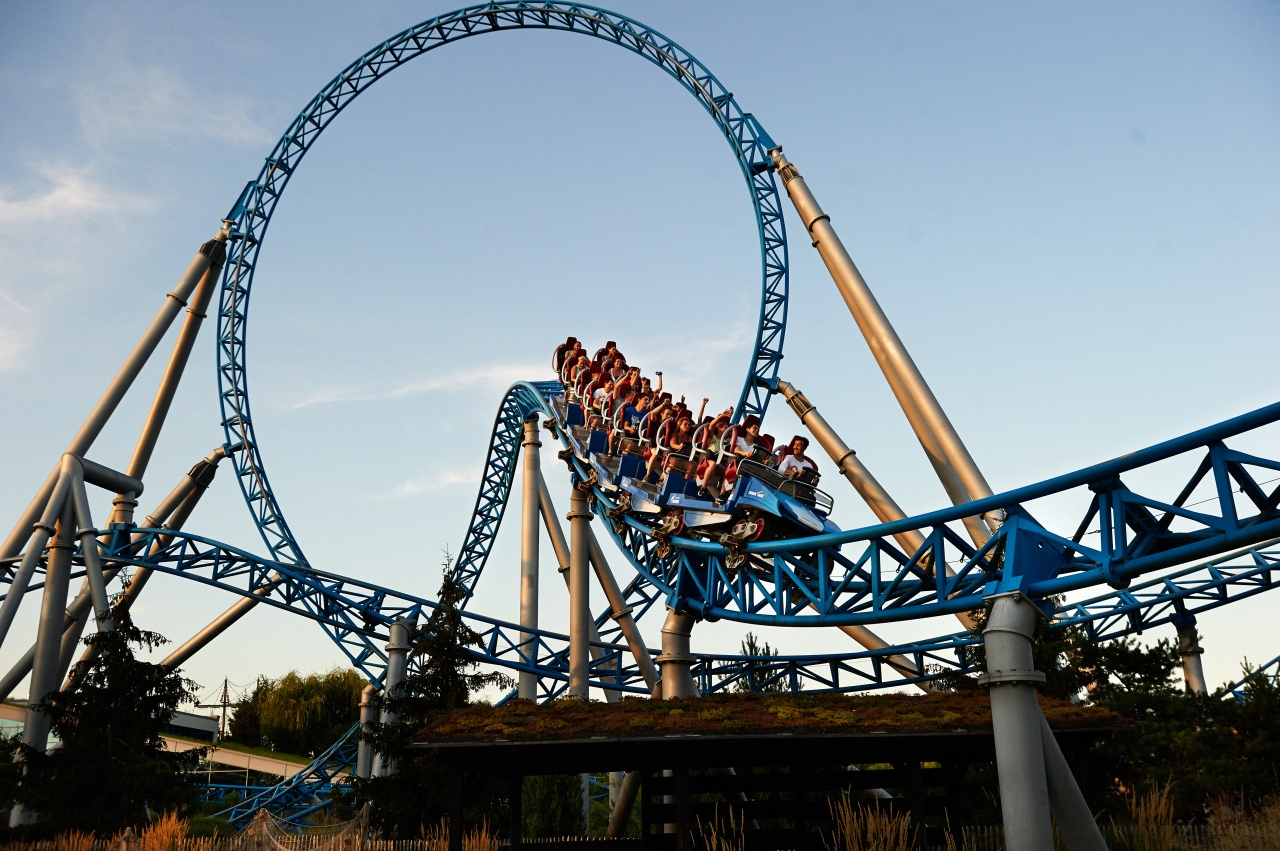
\includegraphics[width=.7\columnwidth]{img/montagnarussa.jpg}
\end{figure}
Immaginiamo una montagna russa ideale, cioè senza attriti di alcun tipo e proponiamone uno schema semplificato.
\end{frame}



\begin{frame}
  \frametitle{Somma costante}
  \begin{figure}
  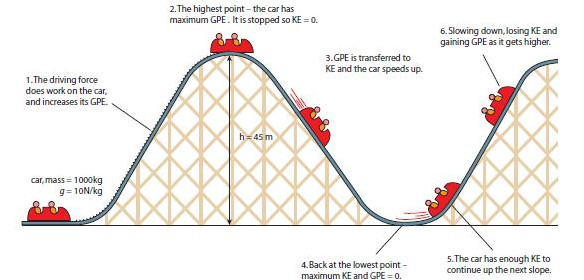
\includegraphics[width=.8\columnwidth]{img/conservazione.jpg}
\end{figure}\pause
Si nota che l'energia cinetica e quella potenziale gravitazionale dei carrelli sono diverse in ogni istante, ma \emph{la loro somma è costante}. Chiamiamo tale somma \alert{energia meccanica del sistema}.
\end{frame}


\begin{frame}
  \frametitle{Conservazione dell'energia}
  Immaginiamo un sistema isolato (su cui non agiscono forze esterne) in cui tutte le forze interne sono conservative.\\~\pause\\  
  Se passiamo da una certa situazione iniziale $ A $ ad una certa situazione finale $ B $, possiamo affermare che \alert<2>{l'energia meccanica totale di un sistema isolato si conserva}:
\begin{center}
\colorbox{blue!30}{$ U_A + K_A = U_B + K_B $}
\end{center}\pause
Questo vale anche per le altre forme di energia possibili:
\begin{block}{Principio di conservazione dell'energia}
  In un sistema isolato l'energia totale si conserva.
\end{block}
\end{frame}



\begin{frame}
\frametitle{Trasferimento di energia}
  Quando una persona salta verso l'alto, essa possiede una certa velocità iniziale, e quindi una certa energia cinetica. Salendo, il lavoro della forza peso \emph<1>{diminuisce l'energia cinetica}, mentre \emph<1>{aumenta l'energia potenziale gravitazionale}.\\~\pause\\In questo e in altri casi, \alert<2>{il lavoro di una forza permette di trasformare una forma di energia in un'altra}.\pause
\begin{block}{Trasferimento di energia}
Il lavoro non è energia, ma è energia in transito (da una forma ad un'altra).
\end{block}
\end{frame}



\begin{frame}
  \frametitle{Esempio}
  \begin{exampleblock}{Conservazione dell'energia durante una caduta}
{\small Un vaso di massa $ 3,00 \, kg $ viene fatto cadere da un'altezza $h = 15,0 \, m $. Una volta raggiunto il suolo, esso rimbalza su una pedana sostenuta da una molla con costante elastica $ 16,0 \, \frac{kN}{m} $.

Calcola:
\begin{itemize}
  \item la velocità con cui il vaso raggiunge la pedana;
  \item di quanto viene compressa la molla.
\end{itemize}}
\end{exampleblock}
\end{frame}

\end{document}
